\documentclass[border=0pt]{standalone}
%\documentclass[onecolumn,journal]{IEEEtran}
%\documentclass[a4paper]{article}

\usepackage{amsmath,epstopdf}

\usepackage{graphicx}
\usepackage{tikz}
\usetikzlibrary{matrix,arrows,shapes,automata}
%% The amssymb package provides various useful mathematical symbols
\usepackage{amssymb}
%% The amsthm package provides extended theorem environments
 \usepackage{amsthm}
 \usepackage{mathrsfs}



\usepgflibrary{shapes.symbols}    
\usepgflibrary[shapes.symbols]    
\usetikzlibrary{shapes.symbols}  
\usetikzlibrary[shapes.symbols]  


\begin{document}

% \begin{figure}
% \centering
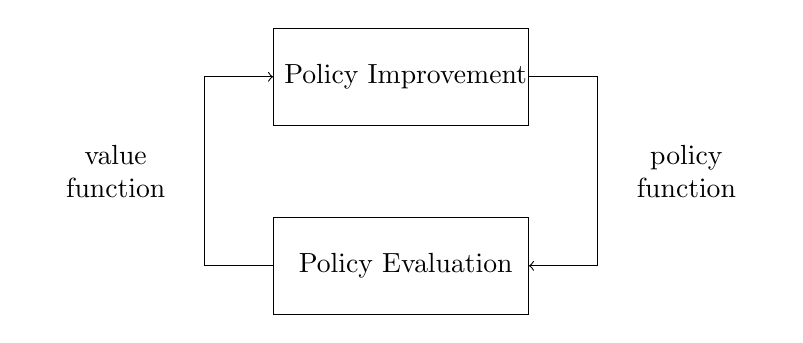
\begin{tikzpicture}
\node [draw, rectangle,  text width=3cm, text height=1cm] (sys1) at (0,1.2) {};
\node [draw, rectangle,  text width=3cm, text height=1cm] (sys2) at (0,-1.2) {};

\node [] at (0,1.2) {{ Policy Improvement}};
\node [] at (0,-1.2) {{ Policy Evaluation}};


%    \node [draw, rectangle,  text width=3cm, text height=1cm, anchor=base] (sys1) {{\Large system 1}};
%    \node [draw, rectangle, below of=sys1,  text width=3cm] (sys2) {{\Large system 2}};   
%
%
%   \draw [->]   (sys1)  |- (sys2);
%%        \draw [->]   (sys2)  |- (sys1);
\draw [->] (sys1) to node[text centered, above]{}(2.5,1.2) to node[text centered, right, text width=2cm]{policy function}(2.5,-1.2) to  (sys2);
\draw [->] (sys2) to node[text centered, below]{}(-2.5,-1.2) to node[text centered, left, text width=2cm] {value function}(-2.5,1.2) to (sys1);
%\draw [->] (-2.5,1.6) to [yshift=6](sys1);


  \end{tikzpicture}
% \end{figure}


\end{document}